\documentclass[hyperref={pdfpagelabels=false}]{beamer}

\usepackage{listings}
\usepackage{algorithm}
\usepackage{ulem}
\usepackage{algorithmicx}
\usepackage{algpseudocode}

\normalem

\usetheme{Warsaw}
\setbeamercovered{transparent}
\setbeamertemplate{footline}[page number]
\setbeamertemplate{navigation symbols}{} %remove navigation symbols
\setbeamertemplate{bibliography entry title}{}

\newcommand{\codestyle}{\small\sffamily}

% "define" Scala
\lstdefinelanguage{scala}{
  alsoletter={@,=,>},
  morekeywords={abstract, case, catch, class, def, do, else, extends, false, final, finally, for, if, implicit, import, match, new, null, object, 
override, package, private, protected, requires, return, sealed, super, this, throw, trait, try, true, type, val, var, while, with, yield, domain, 
postcondition, precondition,invariant, constraint, assert, forAll, in, _, return, @generator, ensure, require, holds, ensuring,=>},
  sensitive=true,
  morecomment=[l]{//},
  morecomment=[s]{/*}{*/},
  morestring=[b]"
}
\lstset{
%  frame=tb,
  language=scala,
%  aboveskip=3mm,
%  belowskip=3mm,
%  lineskip=-0.1em,
  showstringspaces=false,
  columns=fullflexible,
  mathescape=true,
  numbers=none,
  numberstyle=\tiny,
  basicstyle=\codestyle
} 

\newcommand\highlight[1]{\color{red}{#1}}

\begin{document}
\title{Insane: Precise and Compositional Effect Analysis of Higher-Order Programs}
\author{Etienne Kneuss}
\date{\today}

\nocite{*}

\institute[EPFL]{
Laboratory for Automated Reasoning and Analysis \\
School of Computer and Communication Sciences\\
EPFL\\
}

\begin{frame}
    \titlepage
\end{frame}

%\section*{Outline}
%\begin{frame}
%    \frametitle{Outline}
%    \tableofcontents
%\end{frame}

\section{Introduction}

\begin{frame}[label=overview]
    \begin{figure}[t]
        
\includegraphics[width=60mm]{../../../logo.png}\\
        Interprocedural Static Analysis Engine for Scala
    \end{figure}

    \begin{itemize}
        \item Precise pointer and effect analysis
            \begin{itemize}
                \item Interprocedural
                \item Flow sensitive
                \item No annotations required
                \item Compositional
                \item Flexible representation of effects
                \item Designed for higher-order functions
            \end{itemize}
    \end{itemize}
\end{frame}

\begin{frame}
\frametitle{End Goal}
    Statically compute compositional summaries of
    \begin{enumerate}
        \item memory effects
        \item aliasing relations
    \end{enumerate}

    \vspace{25pt}
    For each method, we want to compute a summary that, given an abstract heap
    before the call, will allow the computation of a sound yet precise abstract
    heap after the call.
\end{frame}

\begin{frame}
\frametitle{Abstract Heaps}
  \begin{columns}
    \begin{column}{0.4\textwidth}

        Abstract Heaps: $H$
        \begin{itemize}
            \item Nodes are objects
            \item Edges are fields
        \end{itemize}

        \vspace{10pt}
        Method Summary:
        $S : (H, Par) \rightarrow (H, Ret)$


    \end{column}
    \begin{column}{0.6\textwidth}
      \begin{figure}[t]
            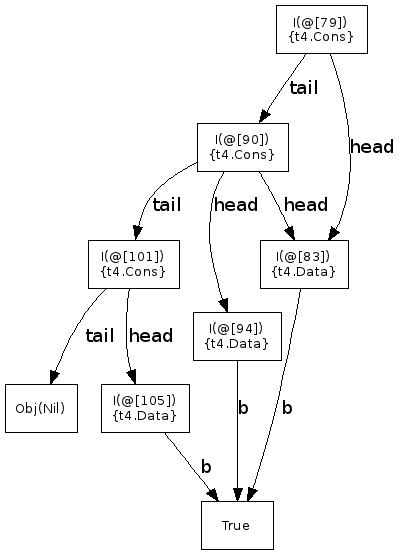
\includegraphics[height=60mm]{images/aheap.png}\\
      \end{figure}
    \end{column}
  \end{columns}
\end{frame}

\begin{frame}
\frametitle{Simple Method Summaries: Requirements}
  Summaries are represented as graphs.

  \vspace{15pt}
  They express how the heap changed, and may refer to values that were
  only reachable before the method call.

  \vspace{15pt}
  They refer to objects that are unknown at the moment: parameters, \emph{this}.

\end{frame}
\subsection{Representation}

\begin{frame}[fragile]
\frametitle{Simple Example}
  \begin{columns}
    \begin{column}{0.4\textwidth}
\begin{lstlisting}
class LList(var data: Int,
           var next: LList)

object Test {
  def run(ll1: LList,
          ll2: LList): LList = {
    val old = ll1.next
    ll1.next = ll2
    old
  }
}
\end{lstlisting}
    \end{column}
    \begin{column}{0.6\textwidth}
      \begin{figure}[t]
            %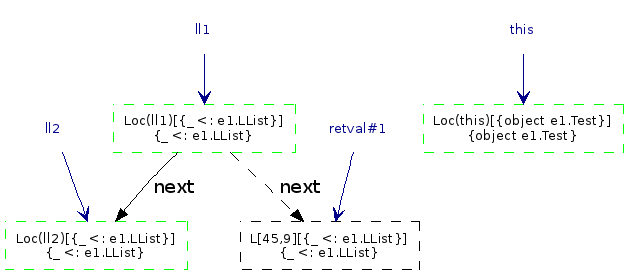
\includegraphics[width=60mm]{images/e1.png}\\
      \end{figure}
    \end{column}
  \end{columns}
\end{frame}

\begin{frame}[fragile]
\frametitle{Simple Example}
  \begin{columns}
    \begin{column}{0.4\textwidth}
\begin{lstlisting}
class LList(var data: Int,
           var next: LList)

object Test {
  def run(ll1: LList,
          ll2: LList): LList = {
    val old = ll1.next
    ll1.next = ll2
    old
  }
}
\end{lstlisting}
    \end{column}
    \begin{column}{0.6\textwidth}
      \begin{figure}[t]
        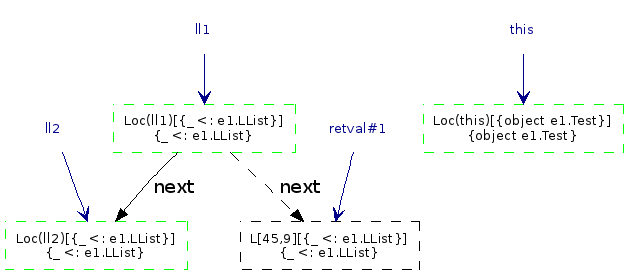
\includegraphics[width=60mm]{images/e1.png}\\
        Test.run()
      \end{figure}
    \end{column}
  \end{columns}
\end{frame}

\begin{frame}[fragile]
\frametitle{Simple Example}
  \begin{columns}
    \begin{column}{0.4\textwidth}
\begin{lstlisting}
object Test {
  def run(ll1: LList,
          ll2: LList): LList = {
    val old = ll1.next
    ll1.next = ll2
    old
  }

  def test() = {
    val ll = new LList(0,
              new LList(1,
               null))
    run(ll, ll)
    ll
  }
}
\end{lstlisting}
    \end{column}
    \begin{column}{0.6\textwidth}
      \begin{figure}[t]
%        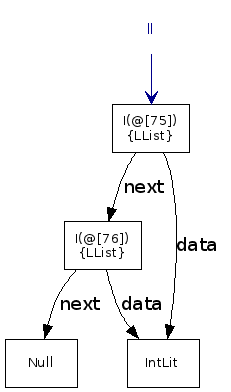
\includegraphics[height=40mm]{images/e1-bef.png}\\
%        Test.test(), before run()
      \end{figure}
    \end{column}
  \end{columns}
\end{frame}

\begin{frame}[fragile]
\frametitle{Simple Example}
  \begin{columns}
    \begin{column}{0.4\textwidth}
\begin{lstlisting}
object Test {
  def run(ll1: LList,
          ll2: LList): LList = {
    val old = ll1.next
    ll1.next = ll2
    old
  }

  def test() = {
    val ll = new LList(0,
              new LList(1,
               null))
    run(ll, ll)
    ll
  }
}
\end{lstlisting}
    \end{column}
    \begin{column}{0.6\textwidth}
      \begin{figure}[t]
        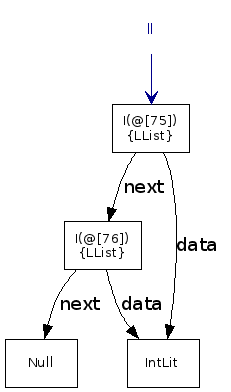
\includegraphics[height=40mm]{images/e1-bef.png}\\
        Test.test(), before run()
      \end{figure}
    \end{column}
  \end{columns}
\end{frame}

\begin{frame}[fragile]
\frametitle{Simple Example}
  \begin{columns}
    \begin{column}{0.4\textwidth}
\begin{lstlisting}
object Test {
  def run(ll1: LList,
          ll2: LList): LList = {
    val old = ll1.next
    ll1.next = ll2
    old
  }

  def test() = {
    val ll = new LList(0,
              new LList(1,
               null))
    run(ll, ll)
    ll
  }
}
\end{lstlisting}
    \end{column}
    \begin{column}{0.6\textwidth}
      \begin{figure}[t]
        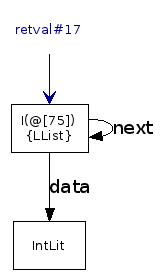
\includegraphics[height=40mm]{images/e1-res.png}\\
        Test.test()
      \end{figure}
    \end{column}
  \end{columns}
\end{frame}

\begin{frame}[fragile]
\frametitle{Method Summaries}
    The method summaries are abstractions:
    \begin{itemize}
        \item not path sensitive
        \item order of writes is lost
        \item we enforce a maximum depth for load nodes
    \end{itemize}
  \begin{columns}
    \begin{column}{0.4\textwidth}
\begin{lstlisting}[escapechar=\%]
  def f(l: LList) = {
    var c = l
    while(c.next != null) {
      c = c.next
    }
    c
  }
\end{lstlisting}
    \end{column}
    \begin{column}{0.6\textwidth}
      \begin{figure}[t]
        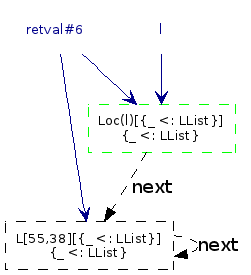
\includegraphics[height=30mm]{images/e6.png}\\
      \end{figure}
    \end{column}
  \end{columns}
\end{frame}

\begin{frame}[fragile]
\frametitle{First Challenge}
\begin{lstlisting}[escapechar=\%]
class LList(var data: Int,
           var next: LList) {
  def mapHead(f: %\highlight{Int $\Rightarrow$ Int}%) = {
    LList(%\highlight{f(data)}%, next)
  }
}
\end{lstlisting}

    \vspace{10pt}
    How can we summarize \emph{mapHead()}?
\end{frame}

\begin{frame}[fragile]
\frametitle{First Challenge}
\begin{lstlisting}[escapechar=\%]
class LList(var data: Int,
           var next: LList) {
  def mapHead(f: %\highlight{F1[Int, Int]}%) = {
    LList(%\highlight{f.apply(data)}%, next)
  }
}
\end{lstlisting}

    \vspace{10pt}
    How can we summarize \emph{mapHead()}?
\end{frame}

\begin{frame}[fragile]
\frametitle{First Challenge}
    Two alternatives: 
    \vspace{15pt}

    \textbf{1: Considering all defined targets:}\\
    \vspace{5pt}
    Bad idea: it kills precision. ($>$1K targets in the library)

    \begin{figure}[t]
        \includegraphics[height=50mm]{images/hist.png}\\
    \end{figure}

\end{frame}

\begin{frame}[fragile]
\frametitle{First Challenge}
    \textbf{2: Delay the analysis of \emph{f.apply}:}\\
    \vspace{5pt}
    Interesting, for such cases:

\begin{lstlisting}[escapechar=\%]
    def plop(l: List) = {
      l.mapHead({ i $\Rightarrow$ i + 1})
    }
\end{lstlisting}

 But how can we record the call left dangling in the effect summary?
\end{frame}

\begin{frame}[fragile]
\frametitle{First Challenge: Delaying}
\begin{lstlisting}[escapechar=\%]
class C(var field1: C, var field2: C);
\end{lstlisting}

\begin{lstlisting}[escapechar=\%]
def plop1(obj: C, f: C $\Rightarrow$ Unit) = {
    obj.field1 = ..
    %\highlight{f(obj)}%
}

def plop2(obj: C, f: C $\Rightarrow$ Unit) = {
    %\highlight{f(obj)}%
    obj.field1 = ..
}
\end{lstlisting}
    \begin{figure}
    \center{
    $S(plop1) =^? S(plop2)$
\pause
\\
\textbf{no}, we want flow-sensitivity
\pause
    \\
    $\Rightarrow$ we need a new representation
    }
    \end{figure}
\end{frame}

\section{New Representation}
\begin{frame}[fragile]
\frametitle{New Effect Representation}
    Instead of generating simple effect graphs we:
    \begin{enumerate}
        \item Start from the CFG,
        \item analyze what we can,
        \item reduce the CFG by introducing \emph{effect statements} summarizing
        blocks of analyzed statements
    \end{enumerate}

    \vspace{15pt}
    \pause

    We obtain a CFG where only dangling method calls remain! We use this
    reduced CFG as summary.

\end{frame}

\begin{frame}[fragile]
\frametitle{Example}
  \begin{columns}
    \begin{column}{0.4\textwidth}
\begin{lstlisting}[escapechar=\%]
class LList(var data: Int,
           var next: LList) {
  def mapHead(f: F1[Int, Int]) = {
    new LList(f.apply(data), next)
  }
}
\end{lstlisting}
    \end{column}
    \begin{column}{0.6\textwidth}
      \begin{figure}[t]
%        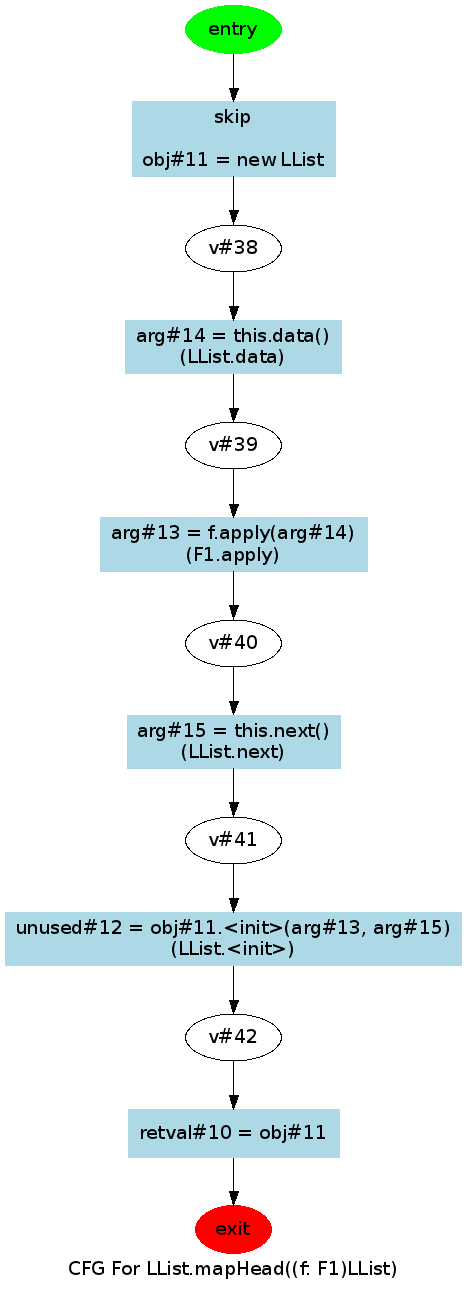
\includegraphics[height=60mm]{images/e3.png}\\
      \end{figure}
    \end{column}
  \end{columns}
\end{frame}
\begin{frame}[fragile]
\frametitle{Example}
  \begin{columns}
    \begin{column}{0.4\textwidth}
\begin{lstlisting}[escapechar=\%]
class LList(var data: Int,
           var next: LList) {
  def mapHead(f: F1[Int, Int]) = {
    val ll = new LList
    ll.<init>(f.apply(this.data()), this.next())
    ll
  }
}
\end{lstlisting}
    \end{column}
    \begin{column}{0.6\textwidth}
      \begin{figure}[t]
        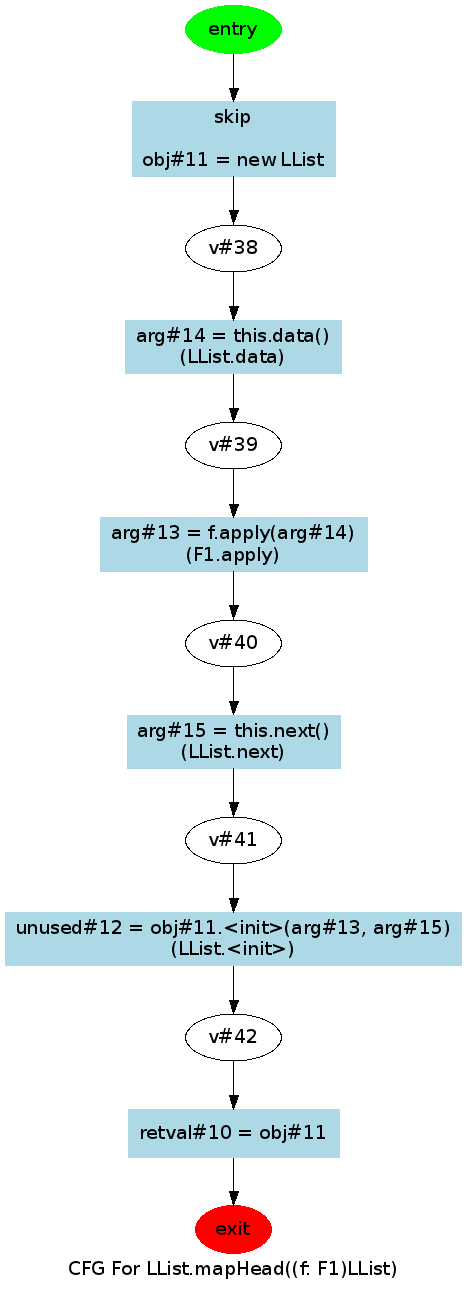
\includegraphics[height=60mm]{images/e3.png}\\
      \end{figure}
    \end{column}
  \end{columns}
\end{frame}

\begin{frame}[fragile]
\frametitle{Example}
  \begin{figure}[t]
    \begin{center}
    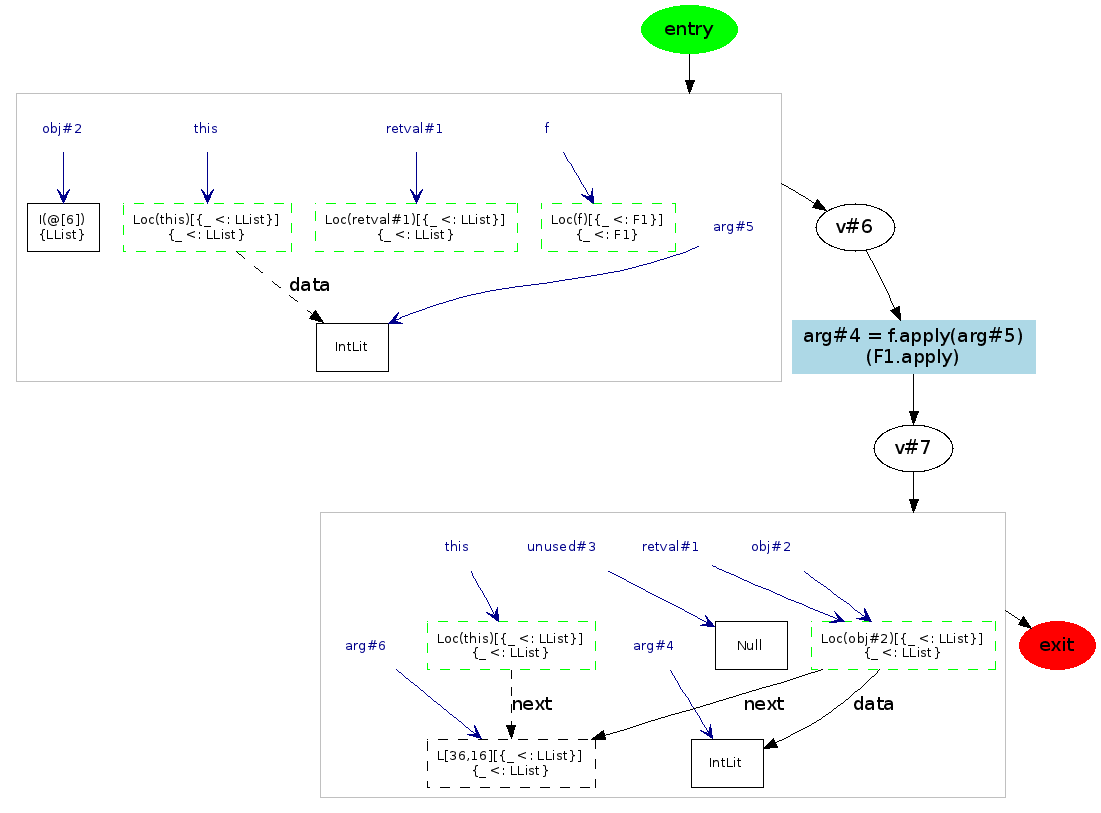
\includegraphics[width=90mm]{images/e4.png}\\
    \end{center}
  \end{figure}
\end{frame}

\begin{frame}[fragile]
\frametitle{Example}
  \begin{columns}
    \begin{column}{0.4\textwidth}
\begin{lstlisting}[escapechar=\%]
class LList(var data: Int,
           var next: LList) {
  def mapHead(f: F1[Int, Int]) = {
    val ll = new LList
    ll.<init>(f.apply(this.data()), this.next())
    ll
  }
}

object Test {
  def test(l: LList) = {
    l.mapHead({ i $\Rightarrow$ 42 })
  }
}
\end{lstlisting}
    \end{column}
    \begin{column}{0.6\textwidth}
      \begin{figure}[t]
        \begin{center}
        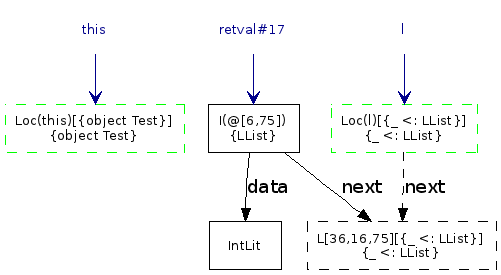
\includegraphics[width=60mm]{images/e5.png}\\
        Test.test()
        \end{center}
      \end{figure}
    \end{column}
  \end{columns}
\end{frame}

\begin{frame}[fragile]
\frametitle{New Effect Representation: Flexibility}
    This representation is very flexible.

    We have at our disposal a very wide spectrum of precision.

    \vspace{15pt}

    \begin{figure}[t]
      \begin{center}
      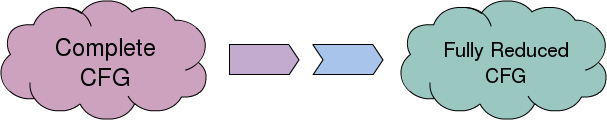
\includegraphics[width=60mm]{images/spectrum.png}\\
      \end{center}
    \end{figure}
\end{frame}

\begin{frame}[fragile]
\frametitle{New Effect Representation: Heuristics}
    How can we automatically decide when to leave the call unanalyzed?

    \vspace{15pt}
    $\Rightarrow$ We rely on score based heuristics.

    \vspace{15pt}
    Multiple ideas on how to compute the score:
    \begin{itemize}
        \item How many targets?
        \item Is the receiver reachable from method arguments?
        \item Can the precision of the receiver improve?
    \end{itemize}
\end{frame}


\section{Conclusions}
\subsection{Current Work}

\begin{frame}[fragile]
\frametitle{Current Work}
    \begin{itemize}
        \item Finalize pipeline modification from \\
            \vspace{5pt}
            ...  $\rightarrow$ explicitOuter $\rightarrow$  erasure $\rightarrow$ lazyVals $\rightarrow$ lambdaLift $\rightarrow$ constructors $\rightarrow$ mixer $\rightarrow$ \textbf{insane}

            \vspace{5pt}
            to \\
            \vspace{5pt}

            ...  $\rightarrow$ explicitOuter $\rightarrow$ \xout{erasure} $\rightarrow$ lazyVals $\rightarrow$ lambdaLift $\rightarrow$ constructors $\rightarrow$ \xout{mixer} $\rightarrow$ \textbf{insane}

        \item By running Insane without erasure, we gain precision and it
        allows us to generate \emph{type-generic summaries}.

    \end{itemize}
\end{frame}

\subsection{Recap}
\begin{frame}[label=overview]
    \begin{figure}[t]
        
\includegraphics[width=60mm]{../../../logo.png}\\
        Interprocedural Static Analysis Engine for Scala
    \end{figure}

    \begin{itemize}
        \item Precise pointer and effect analysis
            \begin{itemize}
                \item Interprocedural
                \item Flow sensitive
                \item No annotations required
                \item Compositional
                \item Flexible representation of effects
                \item Designed for higher-order functions
            \end{itemize}
    \end{itemize}
\end{frame}
\begin{frame}[fragile]
    \begin{figure}
    \begin{center}
    Thanks
    \end{center}
    \end{figure}
\end{frame}
\begin{frame}[fragile]

\frametitle{New Effect Representation: Difficulties}
    There is few difficulties when dealing with CFGs as summaries:
    \begin{itemize}
        \item The CFG under analysis gets modified when inlining the CFG
        corresponding to a method call.\\
            $\Rightarrow$ we discard some of the analysis state and partially restart with the new CFG

        \item The targets of method calls in loops can increase over iterations.\\
            $\Rightarrow$ we cannot simply replace the method call statement with the target CFG

        \item Monotonicity is not ensured in general.\\
            $\Rightarrow$ we have to ensure it by taking specific care of
            recursive methods.
    \end{itemize}
\end{frame}
\end{document}
